

\tikzset{every picture/.style={line width=0.75pt}} %set default line width to 0.75pt        

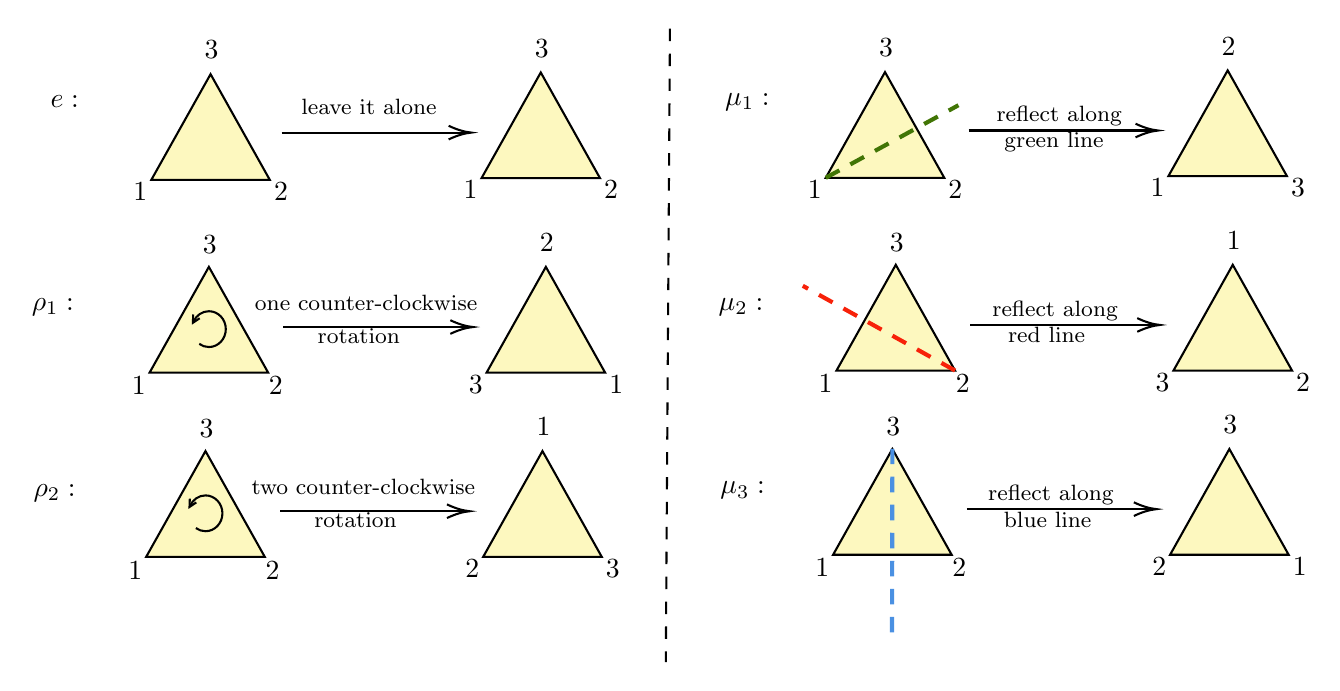
\begin{tikzpicture}[x=0.75pt,y=0.75pt,yscale=-1,xscale=1]
%uncomment if require: \path (0,370); %set diagram left start at 0, and has height of 370

%Shape: Triangle [id:dp770234789038906] 
\draw  [fill={rgb, 255:red, 250; green, 238; blue, 106 }  ,fill opacity=0.43 ] (99.67,41.9) -- (128.22,92.84) -- (71.11,92.84) -- cycle ;
%Shape: Triangle [id:dp3706336221489376] 
\draw  [fill={rgb, 255:red, 250; green, 238; blue, 106 }  ,fill opacity=0.43 ] (258.76,41.08) -- (287.31,92.02) -- (230.2,92.02) -- cycle ;

%Straight Lines [id:da4989662460487787] 
\draw    (133.93,70.05) -- (223.31,70.05) ;
\draw [shift={(225.31,70.05)}, rotate = 180] [color={rgb, 255:red, 0; green, 0; blue, 0 }  ][line width=0.75]    (10.93,-3.29) .. controls (6.95,-1.4) and (3.31,-0.3) .. (0,0) .. controls (3.31,0.3) and (6.95,1.4) .. (10.93,3.29)   ;
%Shape: Triangle [id:dp519914910955628] 
\draw  [fill={rgb, 255:red, 250; green, 238; blue, 106 }  ,fill opacity=0.43 ] (98.85,134.75) -- (127.41,185.69) -- (70.29,185.69) -- cycle ;
%Shape: Triangle [id:dp1396929998067723] 
\draw  [fill={rgb, 255:red, 250; green, 238; blue, 106 }  ,fill opacity=0.43 ] (261.21,134.75) -- (289.76,185.69) -- (232.65,185.69) -- cycle ;

%Straight Lines [id:da9582211177725937] 
\draw    (134.75,163.73) -- (224.12,163.73) ;
\draw [shift={(226.12,163.73)}, rotate = 180] [color={rgb, 255:red, 0; green, 0; blue, 0 }  ][line width=0.75]    (10.93,-3.29) .. controls (6.95,-1.4) and (3.31,-0.3) .. (0,0) .. controls (3.31,0.3) and (6.95,1.4) .. (10.93,3.29)   ;
%Shape: Arc [id:dp48627820726893056] 
\draw  [draw opacity=0] (91.49,161.01) .. controls (92.81,158.11) and (95.61,156.11) .. (98.85,156.11) .. controls (103.36,156.11) and (107.01,159.97) .. (107.01,164.74) .. controls (107.01,169.5) and (103.36,173.37) .. (98.85,173.37) .. controls (97.13,173.37) and (95.53,172.8) .. (94.21,171.84) -- (98.85,164.74) -- cycle ; \draw   (91.49,161.01) .. controls (92.81,158.11) and (95.61,156.11) .. (98.85,156.11) .. controls (103.36,156.11) and (107.01,159.97) .. (107.01,164.74) .. controls (107.01,169.5) and (103.36,173.37) .. (98.85,173.37) .. controls (97.13,173.37) and (95.53,172.8) .. (94.21,171.84) ;  
\draw   (94.43,159.51) -- (91.15,161.67) -- (91.31,157.69) ;

%Shape: Triangle [id:dp7800571980355699] 
\draw  [fill={rgb, 255:red, 250; green, 238; blue, 106 }  ,fill opacity=0.43 ] (97.22,223.49) -- (125.77,274.43) -- (68.66,274.43) -- cycle ;
%Shape: Triangle [id:dp26855524593503344] 
\draw  [fill={rgb, 255:red, 250; green, 238; blue, 106 }  ,fill opacity=0.43 ] (259.58,223.49) -- (288.13,274.43) -- (231.02,274.43) -- cycle ;

%Straight Lines [id:da20079967504625829] 
\draw    (133.12,252.47) -- (222.49,252.47) ;
\draw [shift={(224.49,252.47)}, rotate = 180] [color={rgb, 255:red, 0; green, 0; blue, 0 }  ][line width=0.75]    (10.93,-3.29) .. controls (6.95,-1.4) and (3.31,-0.3) .. (0,0) .. controls (3.31,0.3) and (6.95,1.4) .. (10.93,3.29)   ;
%Shape: Arc [id:dp7942405481223301] 
\draw  [draw opacity=0] (89.86,249.75) .. controls (91.17,246.85) and (93.97,244.85) .. (97.22,244.85) .. controls (101.72,244.85) and (105.38,248.72) .. (105.38,253.48) .. controls (105.38,258.25) and (101.72,262.11) .. (97.22,262.11) .. controls (95.5,262.11) and (93.9,261.54) .. (92.58,260.58) -- (97.22,253.48) -- cycle ; \draw   (89.86,249.75) .. controls (91.17,246.85) and (93.97,244.85) .. (97.22,244.85) .. controls (101.72,244.85) and (105.38,248.72) .. (105.38,253.48) .. controls (105.38,258.25) and (101.72,262.11) .. (97.22,262.11) .. controls (95.5,262.11) and (93.9,261.54) .. (92.58,260.58) ;  
\draw   (92.8,248.25) -- (89.52,250.41) -- (89.67,246.43) ;

%Straight Lines [id:da5406707716678466] 
\draw  [dash pattern={on 4.5pt off 4.5pt}]  (321,20) -- (319,325.18) ;
%Shape: Triangle [id:dp6812685355376344] 
\draw  [fill={rgb, 255:red, 250; green, 238; blue, 106 }  ,fill opacity=0.43 ] (424.61,40.9) -- (453.17,91.84) -- (396.06,91.84) -- cycle ;
%Shape: Triangle [id:dp08881040872765822] 
\draw  [fill={rgb, 255:red, 250; green, 238; blue, 106 }  ,fill opacity=0.43 ] (589.71,40.08) -- (618.26,91.02) -- (561.15,91.02) -- cycle ;

%Straight Lines [id:da3296001217074366] 
\draw    (464.88,69.05) -- (554.25,69.05) ;
\draw [shift={(556.25,69.05)}, rotate = 180] [color={rgb, 255:red, 0; green, 0; blue, 0 }  ][line width=0.75]    (10.93,-3.29) .. controls (6.95,-1.4) and (3.31,-0.3) .. (0,0) .. controls (3.31,0.3) and (6.95,1.4) .. (10.93,3.29)   ;
%Shape: Triangle [id:dp9818559862929847] 
\draw  [fill={rgb, 255:red, 250; green, 238; blue, 106 }  ,fill opacity=0.43 ] (429.8,133.75) -- (458.35,184.69) -- (401.24,184.69) -- cycle ;
%Shape: Triangle [id:dp5966925391786466] 
\draw  [fill={rgb, 255:red, 250; green, 238; blue, 106 }  ,fill opacity=0.43 ] (592.15,133.75) -- (620.71,184.69) -- (563.6,184.69) -- cycle ;

%Straight Lines [id:da7542950918096184] 
\draw    (465.69,162.73) -- (555.07,162.73) ;
\draw [shift={(557.07,162.73)}, rotate = 180] [color={rgb, 255:red, 0; green, 0; blue, 0 }  ][line width=0.75]    (10.93,-3.29) .. controls (6.95,-1.4) and (3.31,-0.3) .. (0,0) .. controls (3.31,0.3) and (6.95,1.4) .. (10.93,3.29)   ;
%Shape: Triangle [id:dp43284317392018445] 
\draw  [fill={rgb, 255:red, 250; green, 238; blue, 106 }  ,fill opacity=0.43 ] (428.16,222.49) -- (456.72,273.43) -- (399.61,273.43) -- cycle ;
%Shape: Triangle [id:dp8956773215716932] 
\draw  [fill={rgb, 255:red, 250; green, 238; blue, 106 }  ,fill opacity=0.43 ] (590.52,222.49) -- (619.08,273.43) -- (561.97,273.43) -- cycle ;

%Straight Lines [id:da21964377356872167] 
\draw    (464.06,251.47) -- (553.44,251.47) ;
\draw [shift={(555.44,251.47)}, rotate = 180] [color={rgb, 255:red, 0; green, 0; blue, 0 }  ][line width=0.75]    (10.93,-3.29) .. controls (6.95,-1.4) and (3.31,-0.3) .. (0,0) .. controls (3.31,0.3) and (6.95,1.4) .. (10.93,3.29)   ;
%Straight Lines [id:da8311353717920538] 
\draw [color={rgb, 255:red, 65; green, 117; blue, 5 }  ,draw opacity=1 ][line width=1.5]  [dash pattern={on 5.63pt off 4.5pt}]  (396.06,91.84) -- (460,56.87) ;
%Straight Lines [id:da06735691218924689] 
\draw [color={rgb, 255:red, 247; green, 33; blue, 9 }  ,draw opacity=1 ][line width=1.5]  [dash pattern={on 5.63pt off 4.5pt}]  (458.35,184.69) -- (385,143.87) ;
%Straight Lines [id:da04188916516791419] 
\draw [color={rgb, 255:red, 74; green, 144; blue, 226 }  ,draw opacity=1 ][line width=1.5]  [dash pattern={on 5.63pt off 4.5pt}]  (428,310.87) -- (428.16,222.49) ;

% Text Node
\draw (61.03,92.64) node [anchor=north west][inner sep=0.75pt]    {$1$};
% Text Node
\draw (128.75,92.64) node [anchor=north west][inner sep=0.75pt]    {$2$};
% Text Node
\draw (95.3,24.44) node [anchor=north west][inner sep=0.75pt]    {$3$};
% Text Node
\draw (141.9,52.62) node [anchor=north west][inner sep=0.75pt]   [align=left] {{\footnotesize leave it alone}};
% Text Node
\draw (220.12,91.82) node [anchor=north west][inner sep=0.75pt]    {$1$};
% Text Node
\draw (287.84,91.82) node [anchor=north west][inner sep=0.75pt]    {$2$};
% Text Node
\draw (254.39,23.62) node [anchor=north west][inner sep=0.75pt]    {$3$};
% Text Node
\draw (60.22,186.31) node [anchor=north west][inner sep=0.75pt]    {$1$};
% Text Node
\draw (126.3,186.31) node [anchor=north west][inner sep=0.75pt]    {$2$};
% Text Node
\draw (94.48,118.11) node [anchor=north west][inner sep=0.75pt]    {$3$};
% Text Node
\draw (119.54,146.86) node [anchor=north west][inner sep=0.75pt]   [align=left] {{\footnotesize one counter-clockwise}\\{\footnotesize  \ \ \ \ \ \ \ \ rotation}};
% Text Node
\draw (256.84,117.29) node [anchor=north west][inner sep=0.75pt]    {$2$};
% Text Node
\draw (290.29,185.49) node [anchor=north west][inner sep=0.75pt]    {$1$};
% Text Node
\draw (222.57,185.49) node [anchor=north west][inner sep=0.75pt]    {$3$};
% Text Node
\draw (58.58,275.05) node [anchor=north west][inner sep=0.75pt]    {$1$};
% Text Node
\draw (124.67,275.05) node [anchor=north west][inner sep=0.75pt]    {$2$};
% Text Node
\draw (92.85,206.85) node [anchor=north west][inner sep=0.75pt]    {$3$};
% Text Node
\draw (117.91,235.6) node [anchor=north west][inner sep=0.75pt]   [align=left] {{\footnotesize two counter-clockwise}\\{\footnotesize  \ \ \ \ \ \ \ \ rotation}};
% Text Node
\draw (255.21,206.03) node [anchor=north west][inner sep=0.75pt]    {$1$};
% Text Node
\draw (288.66,274.23) node [anchor=north west][inner sep=0.75pt]    {$3$};
% Text Node
\draw (220.94,274.23) node [anchor=north west][inner sep=0.75pt]    {$2$};
% Text Node
\draw (21.13,50.73) node [anchor=north west][inner sep=0.75pt]    {$e:$};
% Text Node
\draw (12.05,148.33) node [anchor=north west][inner sep=0.75pt]    {$\rho _{1} :$};
% Text Node
\draw (12.87,237.9) node [anchor=north west][inner sep=0.75pt]    {$\rho _{2} :$};
% Text Node
\draw (385.98,91.64) node [anchor=north west][inner sep=0.75pt]    {$1$};
% Text Node
\draw (453.69,91.64) node [anchor=north west][inner sep=0.75pt]    {$2$};
% Text Node
\draw (420.24,23.44) node [anchor=north west][inner sep=0.75pt]    {$3$};
% Text Node
\draw (476.84,55.62) node [anchor=north west][inner sep=0.75pt]  [font=\footnotesize] [align=left] {reflect along \\ \ green line};
% Text Node
\draw (391.16,185.31) node [anchor=north west][inner sep=0.75pt]    {$1$};
% Text Node
\draw (457.25,185.31) node [anchor=north west][inner sep=0.75pt]    {$2$};
% Text Node
\draw (425.43,117.11) node [anchor=north west][inner sep=0.75pt]    {$3$};
% Text Node
\draw (389.53,274.05) node [anchor=north west][inner sep=0.75pt]    {$1$};
% Text Node
\draw (455.61,274.05) node [anchor=north west][inner sep=0.75pt]    {$2$};
% Text Node
\draw (423.8,205.85) node [anchor=north west][inner sep=0.75pt]    {$3$};
% Text Node
\draw (346.08,49.73) node [anchor=north west][inner sep=0.75pt]    {$\mu _{1} :$};
% Text Node
\draw (343,148.33) node [anchor=north west][inner sep=0.75pt]    {$\mu _{2} :$};
% Text Node
\draw (343.82,236.9) node [anchor=north west][inner sep=0.75pt]    {$\mu _{3} :$};
% Text Node
\draw (586.15,205.03) node [anchor=north west][inner sep=0.75pt]    {$3$};
% Text Node
\draw (619.6,273.23) node [anchor=north west][inner sep=0.75pt]    {$1$};
% Text Node
\draw (551.89,273.23) node [anchor=north west][inner sep=0.75pt]    {$2$};
% Text Node
\draw (587.78,116.29) node [anchor=north west][inner sep=0.75pt]    {$1$};
% Text Node
\draw (621.24,184.49) node [anchor=north west][inner sep=0.75pt]    {$2$};
% Text Node
\draw (553.52,184.49) node [anchor=north west][inner sep=0.75pt]    {$3$};
% Text Node
\draw (585.34,22.62) node [anchor=north west][inner sep=0.75pt]    {$2$};
% Text Node
\draw (618.79,90.82) node [anchor=north west][inner sep=0.75pt]    {$3$};
% Text Node
\draw (551.07,90.82) node [anchor=north west][inner sep=0.75pt]    {$1$};
% Text Node
\draw (474.84,149.62) node [anchor=north west][inner sep=0.75pt]  [font=\footnotesize] [align=left] {reflect along \\ \ \ red line};
% Text Node
\draw (472.84,238.62) node [anchor=north west][inner sep=0.75pt]  [font=\footnotesize] [align=left] {reflect along \\ \ \ blue line};


\end{tikzpicture}
